\documentclass[aspectratio=169]{beamer}
\usetheme{simple}
\usepackage[english]{babel}
\usepackage[utf8]{inputenc} 
\usepackage{lmodern}
\usefonttheme[onlymath]{serif}
\usepackage[scale=2]{ccicons} 
\usepackage[makeroom]{cancel}
\usepackage{copyrightbox}

\usepackage{graphicx,hyperref,url,pgfplots}
\usepackage{amsmath} 
\usepackage{array,booktabs}
\pgfplotsset{compat=1.13}  
\usepackage{pifont}
\usepackage{bibentry}
\usepackage[alf,abnt-etal-list=0,abnt-etal-cite=3]{abntex2cite}
\usepackage[normalem]{ulem}

\setbeamercovered{invisible}
\newcommand{\pausar}{ }
\newcommand{\df}[1]{\,\mathrm{d}#1}
\newcommand{\parcial}[3]{\dfrac{\partial^{#1}#2}{\partial #3^{#1}}}
\newcommand{\cpright}[2]{\copyrightbox[b]{#1}{\tiny Source: #2}}
\newcommand{\cmark}{\textcolor{green}{\ding{51}}}%
\newcommand{\xmark}{\textcolor{red}{\ding{55}}}%

\usepackage{tikz}
\usepackage{xcolor}
\usetikzlibrary{scopes}
\usepackage{verbatim}
\usetikzlibrary{patterns}

\usepackage{listings}
	\definecolor{codegreen}{rgb}{0,0.6,0}
	\definecolor{codegray}{rgb}{0.5,0.5,0.5}
	\definecolor{codepurple}{rgb}{0.58,0,0.82}
	\definecolor{backcolour}{rgb}{0.92,0.92,0.92}
	\lstset{language=Python, 
	backgroundcolor=\color{backcolour},   
	commentstyle=\color{codegreen},
	keywordstyle=\color{magenta},
	numberstyle=\tiny\color{codegray},
	stringstyle=\color{codepurple},
	basicstyle=\fontsize{8}{11}\ttfamily,
	frame=lines,
%	numbers=left,
	tabsize=2,
	morekeywords={models, lambda, forms}}

\usepackage{catchfile}
\newcommand{\getenv}[2][]{%
    \CatchFileEdef{\temp}{"|kpsewhich --var-value #2"}{\endlinechar=-1}%
    \if\relax\detokenize{#1}\relax\temp\else\let#1\temp\fi}

\getenv[\BIBREF]{RM_REFERENCES}

% --------------------------------------------------------------------------------------------

\title{Mobile Robots}
\subtitle{Robot Dynamics}
\date{\today}
\author[Jeferson José de Lima]{
  \textbf{Professor}: Jeferson José de Lima}
  \institute{Academic Department of Informatics (DAINF) \\ Federal University of Technology - Paraná (UTFPR) at Pato Branco, PR, Brazil}

\begin{document}

\maketitle

\begin{frame}{Useful Information}
    \begin{block}{Material disponível em:}
        \href{Robótica Móvel - Wiki}{https://gitlab.com/cursoseaulas/robotica-movel/-/wikis/home}
    \end{block}
    \pausar
    % \begin{block}{Avisos Importantes}
    %     \begin{itemize}
    %         \item \textcolor{red}{Envio Moodle: Nomes das equipes e do Robô}
    %     \end{itemize}
    % \end{block}
    \pausar
    \begin{block}{Materiais e Recursos de Aula}
        \begin{itemize}
            \item Quadros / Slides
            \item Python - Jupyter Notebook (Colab)
        \end{itemize}
    \end{block}
    
\end{frame}


\begin{frame}{Modelagem Cinemática e Dinâmica}
    \framesubtitle{Introdução}
    \begin{itemize}
        \item Modelos:
              \begin{itemize}
                  \item Modelo Cinemático \cmark;
                  \item Modelo Dinâmico;
              \end{itemize}
    \end{itemize}
    \begin{center}
        \cpright{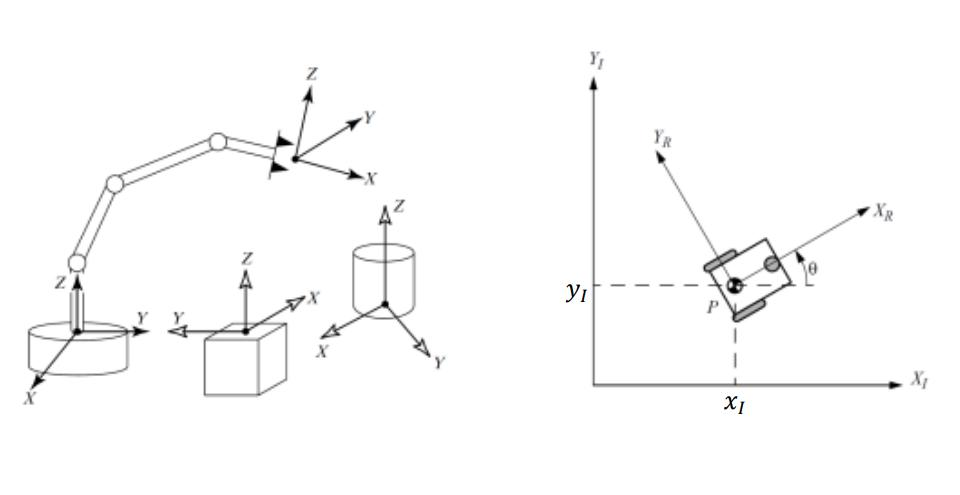
\includegraphics[width=0.8\textwidth]{./images/mecanismos.jpg}}
        {https://edisciplinas.usp.br/pluginfile.php/3280265}
    \end{center}
\end{frame}



\begin{frame}{Dinâmica de Robôs}
    \framesubtitle{Conceito}
    A modelagem dinâmica do robô trata das equações dinâmicas do movimento do robô.
    
    \begin{block}{}
        O \textcolor{red}{modelo cinemático} descreve apenas a \textcolor{red}{transformação estática de algumas velocidades do robô} (pseudo-velocidades) para as velocidades expressas em coordenadas globais. No entanto, o \textcolor{blue}{modelo de movimento dinâmico do sistema mecânico} inclui propriedades dinâmicas, como movimento do sistema causado por \textcolor{blue}{forças externas e inércia do sistema}.
    \end{block}

    \begin{itemize}
        \item \textbf{Método de Euler}
        \item \textbf{Método de Lagrange}
        \begin{itemize}
            \item Sistemas Holonômicos - Sem Restrições de Movimento
            \item Sistemas Não-Holonômicos\footnote[frame]{\textcolor{purple}{Definem-se como não-holonômicos sistemas com dimensão finita onde algum tipo de restrição é imposta a um ou mais estados do sistema.}} - Com Restrições de Movimento
        \end{itemize}
    \end{itemize}
\end{frame}


\begin{frame}{Dinâmica de Robôs - Sistemas Holonômicos}
    \framesubtitle{Coordenadas Generalizadas - Cinemática Inversa e Direta}


    \begin{columns}
        \begin{column}[c]{0.6\textwidth}
            \begin{figure}[!ht]
                

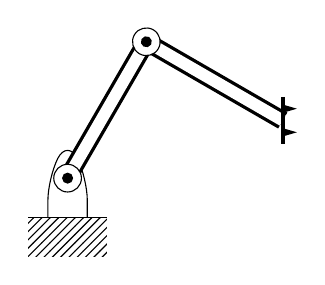
\begin{tikzpicture}
    \newcommand{\nvar}[2]{%
    \newlength{#1}
    \setlength{#1}{#2}
    }

    % Define a few constants for drawing
    \nvar{\dg}{0.3cm}
    \def\dw{0.25}\def\dh{0.5}
    % Define commands for links, joints and such
    \def\link{\draw [double distance=1.5mm, very thick] (0,0)--}
    \def\joint{%
    \filldraw [fill=white] (0,0) circle (5pt);
    \fill[black] circle (2pt);
    }
    \def\grip{%
    \draw[ultra thick](0cm,\dg)--(0cm,-\dg);
    \fill (0cm, 0.5\dg)+(0cm,1.5pt) -- +(0.6\dg,0cm) -- +(0pt,-1.5pt);
    \fill (0cm, -0.5\dg)+(0cm,1.5pt) -- +(0.6\dg,0cm) -- +(0pt,-1.5pt);
    }

    \def\robotbase{%
    \draw[rounded corners=8pt] (-\dw,-\dh)-- (-\dw, 0) --
        (0,\dh)--(\dw,0)--(\dw,-\dh);
    \draw (-0.5,-\dh)-- (0.5,-\dh);
    \fill[pattern=north east lines] (-0.5,-1) rectangle (0.5,-\dh);
    }
    \newcommand{\doublelink}[6]{%
    \robotbase
    \link(#1:#2);
    \joint
    \begin{scope}[shift=(#1:#2), rotate=#1]
        \link(#3:#4);
        \joint
        \begin{scope}[shift=(#3:#4), rotate=#5]
            \grip
        \end{scope}
    \end{scope}
    }

    \doublelink{60}{2}{-90}{2}{-60}{1}
\end{tikzpicture}
    
                \caption{Robô - Dois Graus de Liberdade\footnotemark}
            \end{figure}
        \end{column}
        \begin{column}[c]{0.4\textwidth}
            
            Coordenadas Generalizadas:

            $$
            \color{black}{
                \mathbf{q} = 
                \begin{bmatrix}
                \theta_1 \\
                \theta_2    
                \end{bmatrix}
            }
            $$

            Coordenadas de posição da ferramenta: 

            $$
            \color{blue}{
                \mathbf{x}_{tool} = 
                \begin{bmatrix}
                x_2 \\
                y_2    
                \end{bmatrix}
            }
            $$
        \end{column}
    \end{columns}
\end{frame}


\begin{frame}{Dinâmica de Robôs - Sistemas Holonômicos}
    \framesubtitle{Formulação de Lagrange}

    \begin{itemize}

        \item Equilíbrio de Energias - Formulação de Lagrange:

              \begin{equation}
                  \mathcal{L}= \mathcal{T} - \mathcal{V}
              \end{equation}

        \item A equação de energia cinética ($\mathcal{T}$) é dada por:

            \begin{equation}
                \mathcal{T} = \frac{1}{2} \sum\limits_{k=1}^{N}{\mathbf{\dot{q}}_k}^T  \mathbf{M}_k {\mathbf{\dot{q}}_k}+ \frac{1}{2} \sum\limits_{k=1}^{N}\mathbf{\omega}_k^T \mathbf{J}_k \mathbf{\omega}_k
            \end{equation}

        \item A equação de Energia Potencial Gravitacional($\mathcal{V}_g$) é dada por\footnote{Depende do típo de energia potencial do sistema, neste caso - gravitacional}

            \begin{equation}
                \mathcal{V}_g = \sum\limits_{k=1}^{N}\mathbf{M}g\Delta \underbrace{y_k}_{\text{altura}}
            \end{equation}  


              \begin{block}{}
                  \scriptsize{
                      onde:
                      \begin{tabular}{l|l}
                          $\mathbf{M}$               & Massa              \\
                          $\mathbf{\omega}$ & Velocidade Angular \\
                          $\mathbf{J}$               & Inércia         \\
                      \end{tabular}}
              \end{block}
    \end{itemize}
\end{frame}



\begin{frame}{Dinâmica de Robôs - Sistemas Holonômicos}
    \framesubtitle{Formulação de Lagrange}

    \begin{itemize}
        \item Para Sistemas Holonômicos:
              \begin{equation}
                  \frac{d}{\df{t}}\left( \parcial{}{\mathcal{L}}{\dot{q}_k}\right)
                  -\parcial{}{\mathcal{L}}{q_k}
                  = f_k, \quad k = 1,2,...,n
              \end{equation}

    \end{itemize}
    \begin{block}{}
        onde $k$ é o index das coordenadas generalizadas de $g_k$, $f_k$ são as forças externas que agem no sistema .
    \end{block} 
\end{frame}


\begin{frame}{Dinâmica de Robôs - Sistemas Holonômicos}
    \framesubtitle{Formulação de Lagrange}
    \begin{itemize}
        \item O modelo dinâmico de um robô móvel sem restrições de movimento pode ser expresso pelo sistema de matrizes abaixo:

              \begin{equation}
                  \mathbf{M(q)\ddot{q}+ C(q, \dot{q})+ \color{red}{F(\dot{q})}\color{gray}+G(q) = E(q)u}
              \end{equation}
    \end{itemize}

    \begin{block}{}
        \scriptsize{
            onde:
            \begin{tabular}{ r | l }
                $\mathbf{q}$               & Vetor das coordenadas generalizadas   \\
                $\mathbf{M(q)}$            & Matriz de massa e inercia             \\
                $\mathbf{C(q, \dot{q})}$   & Vetor de força Coriolis e centrifuga  \\
                $\color{red}{\mathbf{F(\dot{q})}}$      & Vetor de atrito, força não conservativa\footnotemark\\
                $\mathbf{G(q)}$            & Vector da força gravitacional         \\
                $\mathbf{E(q)}$            & Matriz dos tranformação dos atuadores \\
                $\mathbf{u}$               & Vetor de entrada                      \\
            \end{tabular}}
    \end{block}
    \footnotetext{As forças que não fazem parte do balanço de energia no formalismo de lagrange, devem ser adicionadas a posteriori no sistema de equações}
\end{frame}


\begin{frame}{Dinâmica de Robôs - Sistemas Holonômicos}
    \framesubtitle{Formulação de Lagrange - Simulação}
    \begin{itemize}
        \item A solução numérica pode ser dada através da integração da aceleração ($\mathbf{\ddot{q}}$):
    \end{itemize}
    \begin{equation}
        \mathbf{\ddot{q}}=\mathbf{M(q)}^{-1}\left\{\mathbf{-C(q, \dot{q})-F(\dot{q})-G(q) + E(q)u}\right\}
    \end{equation}

    \begin{block}{Em espaço de estados}
        \begin{itemize}
            \item Dito isso, o sistema precisa ser expresso em equações de estado.
        \end{itemize}


        \begin{equation*}
            \mathbf{X} = 
            \begin{bmatrix}
                \mathbf{q_1 q_2, \dot{q}_1, \dot{q}_2}.  
            \end{bmatrix}
        \end{equation*}
    \end{block}
\end{frame}


\begin{frame}[fragile]{Dinâmica de Robôs - Sistemas Holonômicos}
    \framesubtitle{Formulação de Lagrange - Simulação}
    Exemplo - Criando o Modelo
	\begin{lstlisting}[language=Python]
    def robot(t,X):
        q1  = X[0]
        q2  = X[1]
        dq1 = X[2] 
        dq2 = X[3]
        # Inertial matrix
        Mq = np.array([...]) 
        # C Matrix
        Cq = np.array([...])
        # Gravitational matrix 
        Gq = np.array([...])
        # Friction Force
        ks = 0
        Fa = ks * np.array([[dq1],[dq1]])
        # Atuator
        U_gain =  tau1 = tau2 = 0
        Eu = U_gain * np.array([[tau1],[tau2]])
        # Init Model
        xdot = np.zeros(4,)
        ...
	\end{lstlisting}
\end{frame}



\begin{frame}[fragile]{Dinâmica de Robôs - Sistemas Holonômicos}
    \framesubtitle{Formulação de Lagrange - Simulação}

	\begin{lstlisting}[language=Python]
        ...

        #dinamic
        q2dot = inv(Mq).dot(-Cq-Fa-Gq)
        # states
        xdot[0] = dq1
        xdot[1] = dq2
        xdot[2] = q2dot[0]
        xdot[3] = q2dot[1]

        return xdot
    \end{lstlisting}
    
    \footnotetext{\href{https://colab.research.google.com/github/jefersonjlima/2dof-arm/blob/master/notebook/Robotic_Arm.ipynb}{Exemplo de simulação dinâmica de um robô} }

\end{frame}



\begin{frame}{Dinâmica de Robôs - Sistemas Não-Holonômicos}
    \framesubtitle{Restrições impostas pelas Rodas}
    \begin{figure}
        \cpright{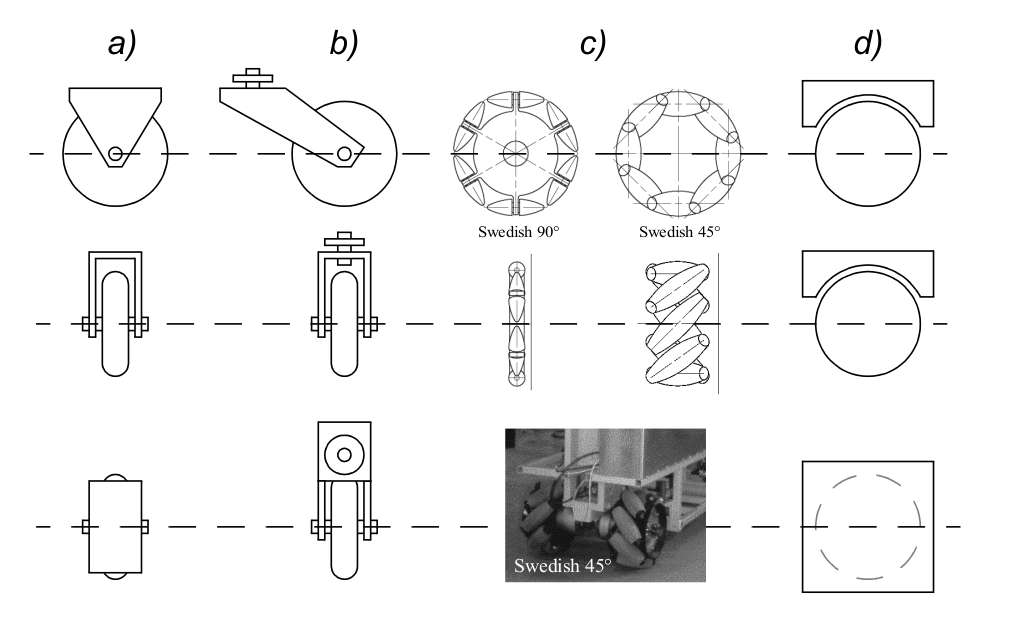
\includegraphics[width=0.8\textwidth]{./images/tipo_de_rodas.png}}
        {\cite{siegwart2011introduction}}
        \caption{ (a) Standard wheel: two degrees of freedom. (b) castor wheel. (c) Swedish wheel: three degrees of freedom. (d) Ball or spherical wheel: realization technically difficult.}
    \end{figure}
\end{frame}

\begin{frame}{Modelo Cinemático}
    \framesubtitle{Robô Diferencial}
    \begin{itemize}
        \item Restrição não-holonômica
              \begin{itemize}
                  \item O robô pode mover-se apenas na direção normal ao eixo das rodas motrizes
              \end{itemize}
              % \begin{equation*}
              %     \dot{x}\sin(\phi) - \dot{y}\cos(\phi) = 0
              % \end{equation*}
        \item As próprias rodas já inserem as restrições!
    \end{itemize}
    \centering
    \def\iangle{35} % Angle of the inclined plane
\def\down{0}
\def\arcr{0.7cm} % Radius of the arc used to indicate angles
\newcommand\centerofmass{%
    \tikz[radius=0.2em] {%
        \fill (0,0) -- ++(0.2em,0) arc [start angle=0,end angle=90] -- ++(0,-0.4em) arc [start angle=270, end angle=180];%
        \draw (0,0) circle;%
    }%
}

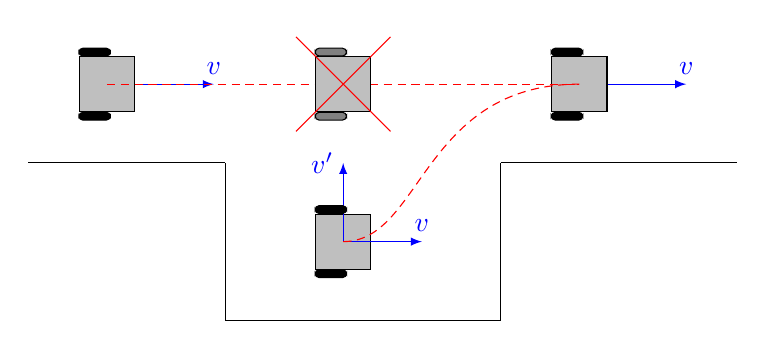
\begin{tikzpicture}[
    force/.style={>=latex,draw=blue,fill=blue},
    axis/.style={densely dashed,gray,font=\small},
    M/.style={rectangle,draw,fill=lightgray,minimum size=0.7cm,thin},
    m/.style={rectangle,draw=black,fill=lightgray,minimum size=0.3cm,thin},
    plane/.style={draw=black,fill=blue!10},
    string/.style={draw=red, thick},
    pulley/.style={thick},
    wheel/.style={fill=black, rounded corners=1.5pt},
]
     \begin{scope}[rotate=0]
        \node[M,transform shape] (M1) at (0,0) {\centerofmass};
        % Draw axes and help lines
        % Forces
        {[force,->]
            % Assuming that Mg = 1. The normal force will therefore be cos(alpha)
            \draw (M1.east) -- ++(1,0) node[above, blue] {$v$};
        }

        \draw[wheel,] (M1.south west) rectangle ++(.4,-.1) node[]{};
        \draw[wheel,] (M1.north west) rectangle ++(.4,.1)  node[]{};
    \end{scope}


    \begin{scope}[rotate=0]
        \node[M,transform shape] (M2) at (6,0) {\centerofmass};
        % Draw axes and help lines
        % Forces
        {[force,->]
            % Assuming that Mg = 1. The normal force will therefore be cos(alpha)
            \draw (M2.east) -- ++(1,0) node[above, blue] {$v$};
        }

        \draw[wheel,] (M2.south west) rectangle ++(.4,-.1) node[]{};
        \draw[wheel,] (M2.north west) rectangle ++(.4,.1)  node[]{};
    \end{scope}
    \begin{scope}[rotate=0]
        \node[M,transform shape] (M3) at (3,-2) {\centerofmass};
        % Draw axes and help lines
        % Forces
        {[force,->]
            % Assuming that Mg = 1. The normal force will therefore be cos(alpha)
            \draw (M3.center) -- ++(1,0) node[above, blue] {$v$};
            \draw (M3.center) -- ++(0,1) node[left, blue] {$v'$};
        }

        \draw[wheel,] (M3.south west) rectangle ++(.4,-.1) node[]{};
        \draw[wheel,] (M3.north west) rectangle ++(.4,.1)  node[]{};
    \end{scope}

%%
    \draw (-1,-1)           -- ++(2.5,0) node[](wall_1){};
    \draw (wall_1.center)   -- ++(0,-2) node[](wall_2){};
    \draw (wall_2.center)   -- ++(3.5,0) node[](wall_3){};
    \draw (wall_3.center)   -- ++(0,2) node[](wall_4){};
    \draw (wall_4.center)   -- ++(3,0) node[](wall_4){};    

    \pausar
    \draw[densely dashed, red] (M1.center) -- (M2.center);
    
    \pausar

    \begin{scope}[rotate=0]
        \node[M,transform shape] (M4) at (3,0) {\centerofmass};
        % Draw axes and help lines
        % Forces

        \draw[wheel,fill=gray] (M4.south west) rectangle ++(.4,-.1) node[]{};
        \draw[wheel,fill=gray] (M4.north west) rectangle ++(.4,.1)  node[]{};

        \draw[red] (3,0) -- ++(-0.6,-0.6) node[]{};
        \draw[red] (3,0) -- ++(0.6,-0.6) node[]{};
        \draw[red] (3,0) -- ++(-0.6,0.6) node[]{};
        \draw[red] (3,0) -- ++(0.6,0.6) node[]{};
    \end{scope}

    \draw[densely dashed, red] (M3.center) .. controls ++(1,0) and ++(-2,0) .. (M2.center);

    % Draw gravity force. The code is put outside the rotated
    % scope for simplicity. No need to do any angle calculations. 
\end{tikzpicture}

\end{frame}


\begin{frame}{Dinâmica de Robôs - Sistemas Não-Holonômicos}
    \framesubtitle{Restrições - Rodas}

    \begin{figure}
        \centering
        \cpright{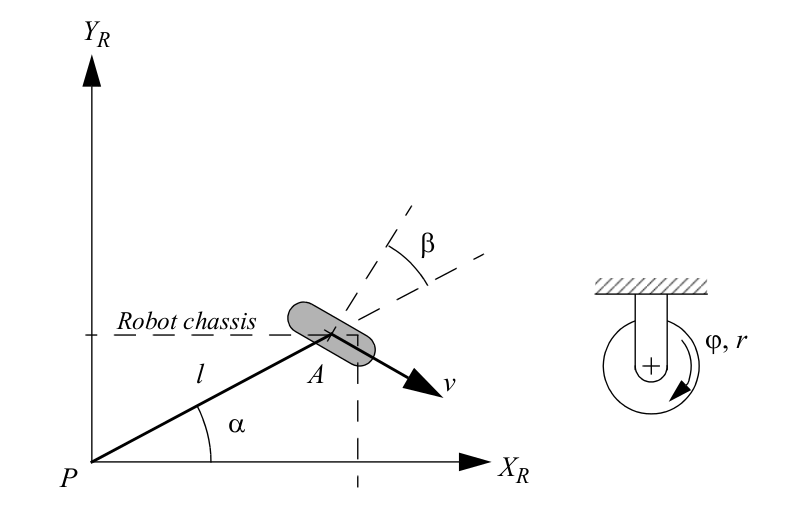
\includegraphics[width=0.6\textwidth]{./images/wheels_const.png}}
        {\cite{siegwart2011introduction}}
        \caption{A fixed standard wheel and its parameters.}
    \end{figure}
\end{frame}


\begin{frame}{Dinâmica de Robôs - Sistemas Não-Holonômicos}
    \framesubtitle{Restrições - Robô Diferencial}

    \centering
    \def\iangle{35} % Angle of the inclined plane
\def\down{0}
\def\arcr{0.7cm} % Radius of the arc used to indicate angles
\newcommand\centerofmass{%
    \tikz[radius=0.2em] {%
        \fill (0,0) -- ++(0.2em,0) arc [start angle=0,end angle=90] -- ++(0,-0.4em) arc [start angle=270, end angle=180];%
        \draw (0,0) circle;%
    }%
}

\begin{tikzpicture}[
    force/.style={>=latex,draw=blue,fill=blue},
    axis/.style={densely dashed,gray,font=\small},
    M/.style={rectangle,draw,fill=lightgray,minimum size=0.7cm,thin},
    m/.style={rectangle,draw=black,fill=lightgray,minimum size=0.3cm,thin},
    plane/.style={draw=black,fill=blue!10},
    string/.style={draw=red, thick},
    pulley/.style={thick},
    wheel/.style={fill=black, rounded corners=1.5pt},
]
    %% Free body diagram of M
    \begin{scope}[rotate=\iangle]
        \node[M,transform shape] (M) {\centerofmass};
        % Draw axes and help lines
        {[axis,->]
            \draw (M) -- ++(0,1.3) node(y1_axis)[right] {$y$};
            \draw (M) -- ++(2,0) node[right] {$x$};
            % Indicate angle. The code is a bit awkward.
            \draw[solid,shorten >=0.5pt] (\down-\iangle:\arcr)
                arc(\down-\iangle:\down:\arcr);
            \node at (\down-0.5*\iangle:1.3*\arcr) {$\phi$};
        }
        % Forces
        {[force,->]
            % Assuming that Mg = 1. The normal force will therefore be cos(alpha)
            \draw (M.east) -- ++(1,0) node[above, blue] {$v_R$};
        }
        \draw[wheel] (M.south west) rectangle ++(.4,-.1) node[below]{$v_{D}$};
        \draw[wheel] (M.north west) rectangle ++(.4,.1)  node[left]{$v_{E}$};
        \draw [dotted, -](M) -- ++(0,2) node(CIR)[above] {CIR};
        \node[below,  yshift=-10, xshift=-5] at (CIR) {$\omega$};
    \end{scope}
    % Draw gravity force. The code is put outside the rotated
    % scope for simplicity. No need to do any angle calculations. 
    \draw[axis,] (M.center) -- ++(1,0) node[below] {};
    %%
    \node[right, gray,font=\small, xshift=8] at (y1_axis) {$\{R\}$};
    %%
    \draw[, ->] (-2,-1) -- ++(4,0) node[below] {$X$};
    \draw[, ->] (-2,-1) -- ++(0,3) node(y_axis)[right] {$Y$};
    \draw[gray, ->] (-2,-1) -- ++(-.5,-.5) node[left] {$Z$};
    \node[left, gray,font=\small, xshift=-10] at (y_axis) {$\{M\}$};
\end{tikzpicture}

    \begin{equation}
        \mathbf{A} = 
        \begin{bmatrix}
            -\sin(\phi) & \cos(\phi) & 0
        \end{bmatrix}
    \end{equation}

\end{frame}


\begin{frame}{Dinâmica de Robôs - Sistemas Não-Holonômicos}
    \framesubtitle{Formulação de Lagrange}

    \begin{itemize}

        \item Equilíbrio de Energias:

              \begin{equation}
                  \mathcal{L}= \mathcal{T} - \mathcal{V}
              \end{equation}

        \item A equação de energia cinética ($\mathcal{T}$) é dada por:

              \begin{equation}
                  \mathcal{T} = \sum\limits_{i=0}^{N-1} \frac{1}{2} {}_{i}^{i+1}\dot{\mathbf{P}}^T\cdot m_{i}\cdot {}_{i}^{i+1}\dot{\mathbf{P}}+ \mathbf{\omega}_i^T\cdot \mathbf{J}_i \cdot \mathbf{\omega}_i
              \end{equation}

              \begin{block}{ou para um robô em uma superfície:}

                  \begin{equation*}
                      \boxed{
                          \mathcal{T} = \frac{m}{2}\left(\dot{x}^2+\dot{y}^2 \right)+ \frac{J}{2}\dot{\phi}^2}
                      \text{, e  }
                      \boxed{\mathcal{V} = 0}
                  \end{equation*}
                  \scriptsize{
                      onde:
                      \begin{tabular}{l|l}
                          $m$               & Massa              \\
                          $\mathbf{\omega}$ & Velocidade Angular \\
                          $J$               & Inércia            \\
                      \end{tabular}}
              \end{block}
    \end{itemize}
\end{frame}




\begin{frame}{Modelo Dinâmico}
    \framesubtitle{Formulação de Lagrange}

    \begin{itemize}
        \item Para Sistemas Holonômicos:
              \begin{equation}
                  \frac{d}{\df{t}}\left( \parcial{}{\mathcal{L}}{\dot{q}_k}\right)
                  -\parcial{}{\mathcal{L}}{q_k}
                  +\tau_{d_k}
                  = f_k, \quad k = 1,2,...,n
              \end{equation}

        \item Para Sistemas Não-Holonômicos \footnote{onde $k$ é o index das coordenadas generalizadas de $g_k$, $P$ representas as energias dissipativas (Atrito),
                  $\tau_d$ representa qualquer disturbio no sistema, $f_k$ são as forças externas que agem no sistema e $a_{jk}$ são os coeficientes das restrições de movimento.}
              \begin{equation}
                  \frac{d}{\df{t}}\left( \parcial{}{\mathcal{L}}{\dot{q}_k}\right)
                  -\parcial{}{\mathcal{L}}{q_k}
                  +\tau_{d_k}
                  = f_k - \sum\limits^{m}_{j=1}\lambda_j a_{jk}
              \end{equation}
    \end{itemize}
\end{frame}


\begin{frame}{Modelo Dinâmico}
    \framesubtitle{Formulação de Lagrange}
    \begin{itemize}
        \item O modelo dinâmico de um robô movel com restrições de movimento pode ser expresso pelo sistema de matrizes abaixo:

              \begin{equation}
                  \mathbf{M(q)\ddot{q}+ C(q, \dot{q})+ F(\dot{q})+G(q) = E(q)u -A}^T\mathbf{(q)}\boldsymbol{\lambda}
              \end{equation}
    \end{itemize}

    \begin{block}{}
        \scriptsize{
            onde:
            \begin{tabular}{ r | l }
                $\mathbf{q}$               & Vetor das coordenadas generalizadas   \\
                $\mathbf{M(q)}$            & Matriz de massa e inercia             \\
                $\mathbf{C(q, \dot{q})}$   & Vetor de força Coriolis e centrifuga  \\
                $\mathbf{F(\dot{q})}$      & Vetor de atrito                       \\
                $\mathbf{G(q)}$            & Vector da força gravitacional         \\
                $\mathbf{E(q)}$            & Matriz dos tranformação dos atuadores \\
                $\mathbf{u}$               & Vetor de entrada                      \\
                $\mathbf{A}^T\mathbf{(q)}$ & Matriz de restrições de movimento     \\
                $\boldsymbol{\lambda}$     & Multiplicador de Lagrange             \\
            \end{tabular}}
    \end{block}
\end{frame}



\begin{frame}{Modelagem Dinâmica}
    \framesubtitle{Formulação de Lagrange - Multiplicador de Lagrange}
    A solução para $\lambda_i$ pode ser encontrada por:
    \begin{itemize}
        \item Método 1: Pseudo-velocidades \cmark
        \item Método 2: Redução de Order \xmark
        \item Método 3: Equações de Euler-Lagrange Modificadas \xmark
        \item Método 4: Calculo das Forças de restrições \xmark
    \end{itemize}
\end{frame}
% http://www.cpdee.ufmg.br/~torres/wp-content/uploads/2018/02/nonholonomic_constraints.pdf


\begin{frame}{Modelagem Dinâmica}
    \framesubtitle{Formulação de Lagrange - Pseudo-velocidades}

    \begin{itemize}
        \item O objetivo é resolver as restrições de $\lambda_i$:

              \begin{equation}\label{eq:rmrestri}
                  \mathbf{M(q)\ddot{q}+ C(q, \dot{q})+ F(\dot{q})+G(q) = E(q)u} - \textcolor{red}{\cancel{\mathbf{A}\mathbf{(q)}^T\boldsymbol{\lambda}}}
              \end{equation}

        \item reelembrando:

              \begin{equation*}
                  \mathbf{\dot{q}} = \mathbf{S}(q)\mathbf{v}
              \end{equation*}

        \item bem como:

              \begin{equation}\label{eq:aprox_accel}
                  \mathbf{\ddot{q}} = \mathbf{\dot{S}}(q)\mathbf{v} + \mathbf{S}(q)\mathbf{\dot{v}}
              \end{equation}

        \item Subustituindo \eqref{eq:rmrestri} em \eqref{eq:aprox_accel} e aplicando a relãção $\mathbf{A}(q)\mathbf{S}(q)=0$, temos a equação de aceleração do sistema:

              \begin{equation}\label{eq:pseudovelo}
                  \mathbf{\dot{v}} = \mathbf{\tilde{M}}^{-1}\left(\mathbf{\tilde{E}u - \tilde{V}} \right)
              \end{equation}
    \end{itemize}
\end{frame}



\begin{frame}{Modelagem Dinâmica}
    \framesubtitle{Formulação de Lagrange - Pseudo-velocidades}
    \begin{itemize}
        \item \eqref{eq:pseudovelo} na forma de equação:
              \begin{equation*}
                  \mathbf{\dot{x}} =
                  \begin{bmatrix}
                      \mathbf{S}(q)\mathbf{v} \\
                      \mathbf{-\tilde{M}}^{-1}\mathbf{\tilde{V}}
                  \end{bmatrix}
                  +
                  \begin{bmatrix}
                      \mathbf{0} \\
                      \mathbf{\tilde{M}}^{-1}\mathbf{\tilde{E}}
                  \end{bmatrix} \mathbf{u}
              \end{equation*}

        \item onde:

              \begin{equation*}
                  \begin{split}
                      \mathbf{\tilde{V}} & =
                      \mathbf{S}(q)^T\mathbf{M}\mathbf{\dot{S}}(q)\mathbf{v} + \mathbf{S}(q)^T (\mathbf{V + F + G})\\
                      \mathbf{\tilde{M}} & = \mathbf{S}(q)^T\mathbf{M}\mathbf{S}(q)\\
                      \mathbf{\tilde{E}} & = \mathbf{S}(q)^T\mathbf{E}\mathbf{S}
                  \end{split}
              \end{equation*}

              \begin{block}{}
                  \scriptsize{
                      onde:
                      \begin{tabular}{ r | l }
                          $\mathbf{x}$ & Vetor de estados \\
                          $\mathbf{S}$ & Matriz Jacobiana \\
                      \end{tabular}}
              \end{block}


    \end{itemize}
\end{frame}



\begin{frame}{Modelagem Dinâmica}
    \framesubtitle{Formulação de Lagrange - Exemplo Robô Diferencial}

    \begin{itemize}
        \item Modelo Dinâmico Robô Diferencial
    \end{itemize}

    \begin{columns}
        \begin{column}[c]{0.4\textwidth}
            \begin{figure}
                \centering
                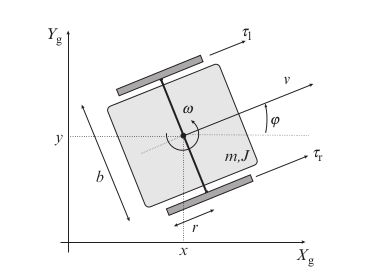
\includegraphics[width=1\textwidth]{./images/dynamic_diff_car.png}
                \caption{Robô Diferencial}
            \end{figure}
        \end{column}
        \begin{column}[c]{0.6\textwidth}
            \begin{equation*}
                \begin{bmatrix}
                    \dot{x} \\ \dot{y} \\ \dot{\phi} \\ \dot{v} \\ \dot{\omega}
                \end{bmatrix}=
                \begin{bmatrix}
                    v \cos(\phi) \\ v \sin(\phi) \\ \omega \\ 0 \\ 0
                \end{bmatrix} + 
                \begin{bmatrix}
                    0 & 0 \\
                    0 & 0 \\
                    0 & 0 \\
                    \frac{1}{mr} & \frac{1}{mr} \\
                    \frac{L}{2Jr} & \frac{-L}{2Jr} \\
                \end{bmatrix}
                \begin{bmatrix}
                    \tau_r \\ \tau_l
                \end{bmatrix}
            \end{equation*}
        \end{column}
    \end{columns}

\end{frame}

\begin{frame}[c]{Exemplo}
    \framesubtitle{Modelagem de um Uniciclo}
    Como descrever o sistema abaixo pelas equacões da cinemática e dinâmica?

    \centering
    \cpright{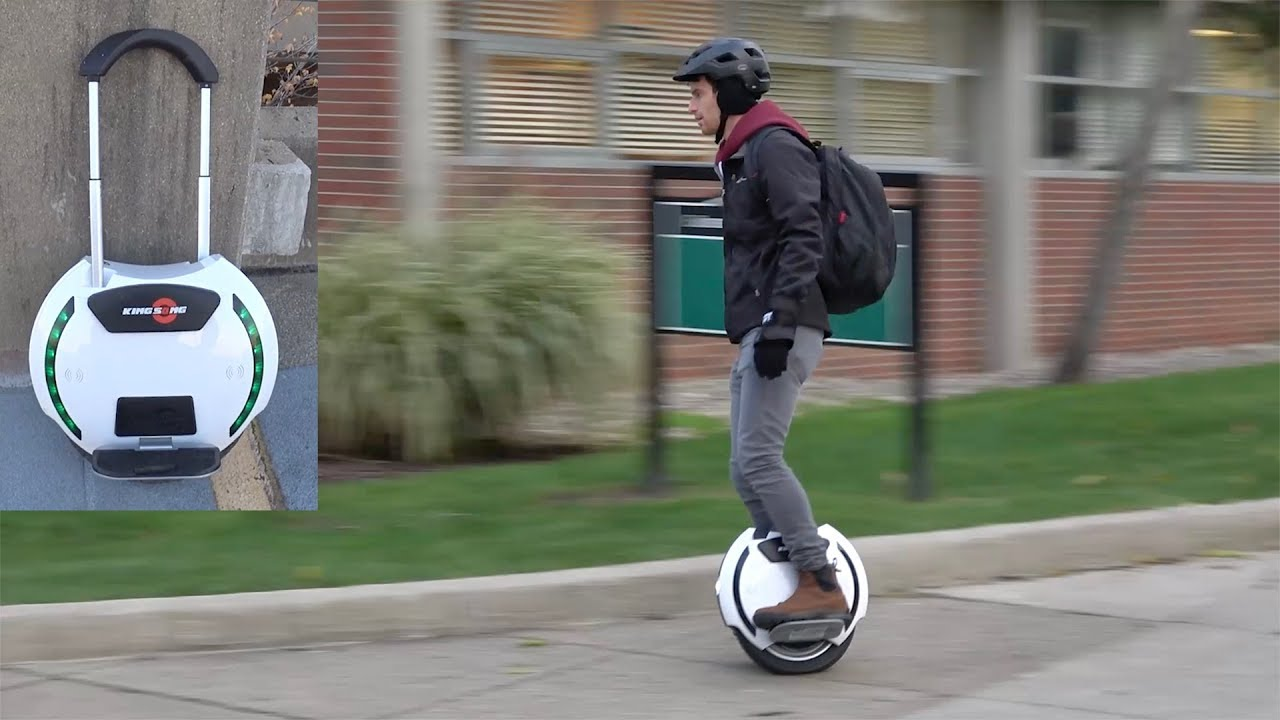
\includegraphics[width=0.8\textwidth]{./images/unicycle.jpg}}
    {https://www.change.org/p/info-theairwheel-com-make-electric-unicycles-legal-to-ease-traffic}
\end{frame}



\begin{frame}[c]{Exemplo}
    \framesubtitle{Modelagem de um Uniciclo}
    \begin{columns}
        \begin{column}[c]{0.4\textwidth}
            \centering
            \scalebox{-1}[1]{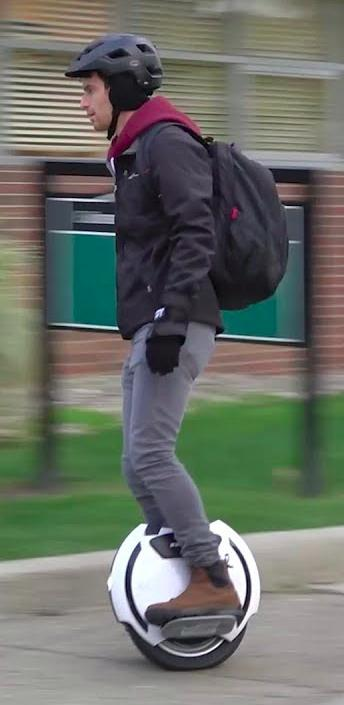
\includegraphics[width=0.6\textwidth]{./images/unicycle_2.jpg}}
        \end{column}
        \begin{column}[c]{0.6\textwidth}
            \centering
            \cpright{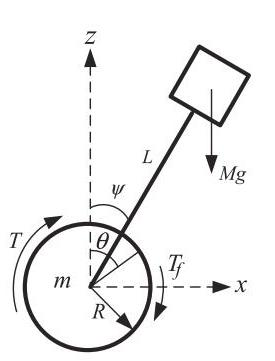
\includegraphics[width=.6\textwidth]{./images/unicycle_model.jpg}}
            {\cite{garcia2017comparative}}
        \end{column}
    \end{columns}
\end{frame}






\begin{frame}[t, allowframebreaks]
	\frametitle{Referências}
	\bibliography{\BIBREF}
\end{frame}
  



\end{document}